\documentclass[a4paper,12pt]{article}
\usepackage[margin=0.7in]{geometry}
\usepackage[latin1]{inputenc}
\usepackage[english]{babel}
\usepackage{amsmath}
\usepackage{cases}
\usepackage[makeroom]{cancel}
\usepackage{amsmath,tabu}
\usepackage[fleqn]{mathtools}
\usepackage[fleqn]{amsmath}
\usepackage{bm}
\usepackage{tikz}
\usepackage{enumitem}
\usepackage{wrapfig}
\usepackage{graphicx}
\usepackage{siunitx}
\usepackage{microtype}
\usepackage{array,tabularx}
\usepackage{float}
\usepackage{booktabs}
\usepackage{import}
\usepackage{cases}
\usepackage{myUnitOfMeasure}
\usepackage{myThermodynamics}
\usepackage{myMath}

\title{PRECEPT 5: Refrigeration cycle}
\author{Rossi Andrea 875272}
\date{}


%\newcommand{\pointdatatable}[5]{
%\begin{center}
%\tabulinesep=1.2mm
%\begin{tabu}{|l|c|c|c|}
%\hline
%$ T_{#1} $ & $ p_{#1} $ & $ h_{#1} $ & $ s_{#1} $\\ \hline
%$ \round{#2} \celsius $ & $ \round{#3} \,bar $ & $ \round{#4} \kjkg $ & $ \round[round-precision=4]{#5} \kjkgk $\\ \hline
%\end{tabu}
%\end{center}
%}

%\newcommand{\Lt}{L_{tubes}}
\newcommand{\Lt}[1][\,]{L^{#1}_{\text{tubes}}}
\newcommand{\It}[1][\,]{I^{#1}_{\text{tubes}}}
\newcommand{\Nt}[1][\,]{N^{#1}_{\text{tubes per row}}}
\newcommand{\Nr}[1][\,]{N^{#1}_{\text{rows}}}
\newcommand{\Tcond}{T_{\text{cond}}}
\newcommand{\Tevap}{T_{\text{evap}}}
\newcommand{\pcond}{p_{\text{cond}}}
\newcommand{\pevap}{p_{\text{evap}}}
\newcommand{\psep}{p_{\text{sep}}}

\renewcommand{\thesubsection}{\thesection.\Alph{subsection}}

%
%
%
%
%
%
%
%
%
%
%
\begin{document}
\maketitle

The refrigeration circuit of a refrigerator for fresh food storage is based on a vapour-compression refrigeration cycle with a single evaporator (with a single lamination valve). The plant has the layout as shown in figure \ref{fig:plant}
\begin{figure}[h]
  \caption{Refrigeration Circuit Layout.}
  \label{fig:plant}
  \centering
    \includegraphics[width=0.5\textwidth]{plant_fig}
\end{figure}

The volumetric compressor is a reciprocating type with single action. 
The condenser consists of a compact tube and fin heat exchanger.

In particular for the refrigerator it is required to: 
\begin{itemize}
\item evaluate the thermodynamic conditions for each point of the cycle for the following condensation temperatures: $30\celsius$, $34\celsius$, $38\celsius$; 
\item draw the plant scheme and the corresponding thermodynamic cycle on (P-h) and (T-s) diagrams, reporting the most relevant thermodynamic points; 
\item calculate the volumetric flow rate at the compressor inlet;
\item calculate the compressor displacement (only for the design condition $\Tcond$ = $30\celsius$);
\item evaluate the thermal power rejected by the condenser; 
\item design the tubes length $\Lt$ for each section of the condenser (de-superheat, condensation and sub-cooling); 
\item calculate the electrical power of the compressor and of the fan; 
\item calculate the coefficient of performance (C.O.P.) of the cycle and of the overall plant;
\item how do the C.O.P. of the cycle varies adopting a double-throttling refrigeration cycle configuration (to be evaluated only for $\Tcond$ = $34\celsius$) assuming as pressure of the vapor-liquid separator (outlet pressure of the first throttling valve) 3,5,7\,bar? Draw the plant scheme and the corresponding thermodynamic cycle on (P-h) and (T-s) diagrams, reporting the most relevant thermodynamic points. 
\end{itemize}

\section{Thermodynamic points}

We need to evaluate the thermodynamic conditions for three different values of $\Tcond$. In the following paragraphs are shown the result for $\Tcond = 34\celsius$, but you can do the same calculations starting with any other values of $\Tcond$. 

\begin{figure}[h]
  \caption{T-s diagram.}
  \label{fig:ts_diagrammA}
  \centering
    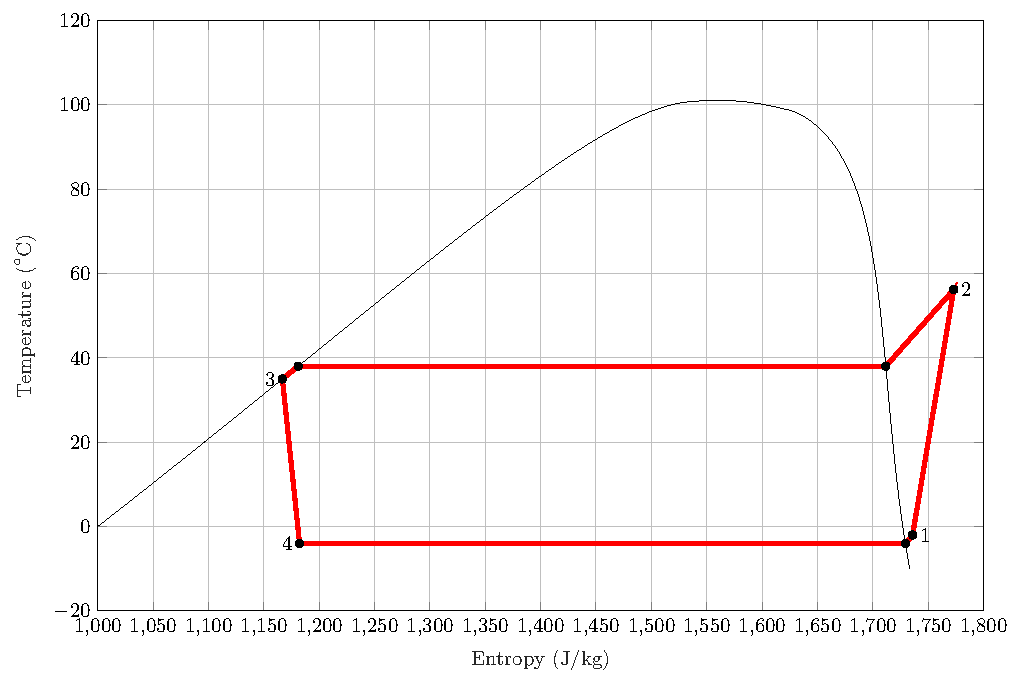
\includegraphics[width=0.8\textwidth]{plot_TS_caseA}
\end{figure}

\begin{figure}[h]
  \caption{p-h diagram.}
  \label{fig:ph_diagrammA}
  \centering
    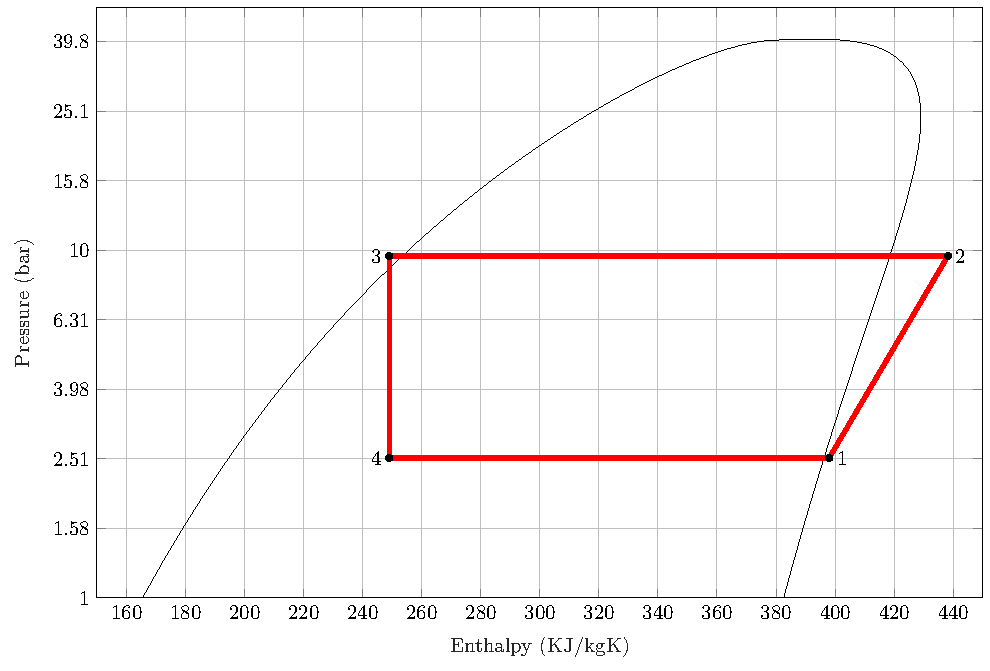
\includegraphics[width=0.8\textwidth]{plot_PH_caseA}
\end{figure}

\subsubsection*{Point 1)}
Point 1 is at \emph{compressor inlet}. We know its temperature $T_1=\Tevap + \Delta\T{SH}$ and its pressure exactly the evaporation pressure $p_1 = p{SAT}(\Tevap)$. With the two parameters of temperature and pressure we can evaluate with \md of R134a also entropy and enthalpy functions of temperature and pressure:
\[\begin{cases}{}
T_1 = \Tevap + \Delta\T{SH} = -4\celsius + 2\celsius = -2\celsius \\ 
p_1 = \p{SAT}(\Tevap) = \round{252675.641745724/100000}\,bar
\end{cases}\]
\pointdatatable{1}{-2}{2.526756417457240}{398.0080526304495}{1.735915384972629}
%
%
%
\subsubsection*{Point 2)}
Point 2 is at \emph{compressor outlet}. We know its pressure $p_2=\pcond\,bar$. We do not directly have the temperature $T_2$ but we can obtain it from the definition of efficiency of the compressor:
\begin{equation}
\label{eq:eta_highp_turbine_iso}
\eta_T^{isoentropic} = \frac{h_2^{IS}-h_1}{h_2-h_1} = 70\%
\end{equation}
We don't know $h_2^{IS}$ but we can compute it from point 1 to point $2^{IS}$ considering an \emph{isoentropic process}:
\[\begin{cases}{}
p_2^{IS} = p_2 = \round{862625.775293017/100000} \,bar \\ 
s_2^{IS} = s_1 = \round{1.735915384972629} \kjkgk
\end{cases}\]
Now we can obtain from \md $h_2^{IS} = h(p_2^{IS},\ s_2^{IS}) = \round{423797.640546623/1000} \kjkg$.
\\Reversing equation \ref{eq:eta_highp_turbine_iso} we can get $h_2$:
\begin{equation}
h_2=h_1- \frac{h_1 - h_2^{IS}}{\eta_T^{iso}} = \round{434850.321082126/1000} \kjkg
\end{equation}
With \md we finally evaluate $s_2 = s(p_2,\ h_2)$ and $T_2 = T(p_2,\ h_2)$ of point 2:
\pointdatatable{2}{324.316135607618-273.15}{862625.775293017/100000}{434850.321082126/1000}{1770.56681577173/1000}
%
%
%
\subsubsection*{Point 3)}
Point 3 is at \emph{condenser outlet}. We know its temperature $T_3=\Tcond - \Delta\T{SC}$ and its pressure exactly the condensation pressure $p_3 = \p{SAT}(\Tcond)$. With the two parameters of temperature and pressure we can evaluate with \md of R134a also entropy and enthalpy functions of temperature and pressure:
\[\begin{cases}{}
T_3 = \Tcond - \Delta\T{SC} = \round{304.15-273.15}\celsius \\ 
p_3 = \p{SAT}(\Tcond) = \round{862625.775293017/100000}\,bar
\end{cases}\]
\pointdatatable{3}{304.15-273.15}{862625.775293017/100000}{243167.202571111/1000}{1148.00179566533/1000}
%
%
%
\subsubsection*{Point 4)}
Point 4 is at \emph{valve outlet}. We can model the valve as \emph{isoenthalpic} so we know enthalpy of point 4 as it is equal to point 3. Moreover we can consider that point 4 is also at evaporator inlet so it is at evaporation pressure. With the two parameters of enthalpy and pressure we can evaluate with \md of R134a also entropy and temperature functions of enthalpy and pressure: 
\[\begin{cases}{}
h_4 = h_3 = \round{243167.202571111/1000}\kjkgk \\ 
p_3 = \pevap = \round{252675.641745724/100000}\,bar
\end{cases}\]
\pointdatatable{4}{269.15-273.15}{252675.641745724/100000}{243167.202571111/1000}{1160.64375010921/1000}
%
%
%

Similarly changing $\pevap$ we get the thermodynamical condition of each point of the plant.

\subimport{tables/}{T30}
\subimport{tables/}{T34}
\subimport{tables/}{T38}

\section{Volumetric flow rate at the compressor inlet}
The volumetric flow rate of a specific point is the mass flow rate of that point divided by its density:
\begin{equation}
\vdot{1} = \dfrac{\mdot{refrigerant}}{\rho_1}
\end{equation}
We have already computed the density of the fluid at the inlet of the compressor, but we miss the mass flow rate; we can evaluate it with an energy balance about the condenser, because we have the useful heat exchanged by the cycle.
\begin{equation}
\Qdot{evap} = \mdot{refrigerant} \cdot (\h{1} - \h{4}) = 18\kw
\qquad \Rightarrow \qquad
\mdot{refrigerant} = \frac{\Qdot{evap}}{\h{1} - \h{4}} = \round{0.112077260245245}\kgs
\end{equation}
Finally we obtain the volumetric flow rate
$\vdot{1} = \frac{\mdot{refrigerant}}{\rho_1} = \round{0.00904240146847206*1000}\,l/s$

\section{Compressor displacement}
We can obtain the compressor displacement from the definition of the volumetric efficiency of the compressor; in fact:
\begin{equation}
\eta_{vol} = \frac{\vdot{1}}{n \cdot V_{cil}}
\qquad \Rightarrow \qquad
V_{cil} = \frac{\vdot{1}}{n \cdot \eta_{vol}} = \round{0.000202971974600944*1000000}\cmcube
\end{equation}

\section{Thermal power rejected by the condenser}
The thermal power rejected by the refrigeration cycle, $\Qdot{cond}$, which has to be discharged in the hot heat sink (the environment) by means of the condenser, results from the application of the \emph{first law of thermodynamics} to the hot side (refrigerant stream) of the condenser. This is a simple task since we already have all the thermodynamical properties for each point, in particular at the inlet and at the outlet of the condenser; 
\begin{equation}
\Qdot{cond} = \mdot{refrigerant} \cdot (\h{2} - \h{3}) = \round{2.174199982378227e+04/1000}\kw
\end{equation} 

\section{Design of the tubes length $\Lt$ for each section of the condenser}
\begin{figure}[h]
  \caption{Condenser Layout.}
  \label{fig:condenser}
  \centering
    \includegraphics[width=0.4\textwidth]{condenser_fig}
\end{figure}
Since the geometry of the heat exchanger is not given, the $\Delta\T{\text{mean\ log}}$ method is easier. In order to use this method the heat exchanger has to be divided based on the heat transfer coefficient values. Depending on which type of fluid we use to transfer heat, sub-cooled water, two phase mixture or super-heated vapour, we have different values of heat transfer coefficient. Even if the coefficient could be different the approach would be almost the same for the three cases.
For this reason we will develop the entire explanation for sub-cooled part and condensation temperature $\Tcond = 34\celsius$and than we will explain the differences for the others.
The scheme of the condenser is represented in figure \ref{fig:condenser}

\subsection*{Sub-cooling condenser}
The heat exchanged in condenser can be written in two different ways:
\begin{equation}
\label{eq:qcond_ref}
\Qdot{cond} = \mdot{refrigerant} \cdot \Delta h = U_{int}A_{int} \cdot \Delta\T{ml} \cdot F
\end{equation}
\begin{conditions*}
U & Heat transfer coefficient;\\[0.5em]
A & Surface of heat transfer;\\[0.5em]
\Delta\T{ml} & Mean log delta temperature;\\[0.5em]
F & Correction factor for an heat exchanger it is not counter current, and it is function of two parameters P
\footnote{\begin{flalign*}
P =& \frac{\T{cold}^{out}-\T{cold}^{in}}{\T{hot}^{in}-\T{cold}^{in}}&
R =& \frac{\T{hot}^{in}-\T{hot}^{out}}{\T{cold}^{out}-\T{cold}^{in}}&
\end{flalign*}}
and R;\\[0.5em]
\end{conditions*}
The surface $A_{int}$ is the lateral surface of a cylinder for each tube so it is function of $\Lt$:
\begin{equation}
A_{int} = \pi D_{int} \cdot \Lt \cdot \Nr \cdot \Nt
\end{equation}
We can also consider the heat exchanged in the air side:
\begin{equation}
\label{eq:qcond_air}
\Qdot{cond} = \mdot{air} \cdot c_{p_{air}} (\T{in} - \T{out})
= \rho_{air} \cdot v_{air} \cdot A_{fin} \cdot c_{p_{air}} (\T{in}^{air} - \T{out}^{air})
\end{equation}
$A_{fin}$ is the frontal surface of the condenser, and it takes into account the thickness of the fins and it is also function of the unknown tube length.
\begin{equation}
A_{fin} = \Lt \cdot \It \cdot \Nt - s_A \left\lfloor \frac{\Lt}{p_A}\right\rfloor \cdot \It \cdot \Nt 
\end{equation}
\begin{conditions}
\Lt & tubes length;\\[0.5em]
\It & tubes pitch;\\[0.5em]
\Nt & number of tubes per row;\\[0.5em]
p_A & fin pitch;\\[0.5em]
\end{conditions}
To evaluate the heat transfer coefficient we apply the series rules of resistance:
\begin{align}
R_{TOT} = \frac{1}{U_{int}A_{int}} = R_{ext} + R_{int} + \cancel{R_{wall}} + R_{fin}
\end{align}
%
The resistance of the wall is small compared to the others so we can neglect it.
\begin{equation}
R_{TOT} = \frac{1}{U_{int}\cancel{A_{int}}} =
\frac{1}{h_{int}\cancel{A_{int}}} + \frac{1}{h_{ext}(\cancel{A_{\text{bare tube}} + A_{fin}}) \cdot \eta_0} 
\end{equation}
We cancel $A_{int}$ with $A_{\text{bare tube}}$ because they are comparable. 
\begin{equation}
U_{int} = \left( \frac{1}{h_{int} + h_{ext} \cdot \eta_0} \right)^{-1} 
= \round{6.235842977439370e+02} \wmsquareK
\end{equation}
Reverting equation \ref{eq:qcond_air} we obtain $\T{out}^{air}$:
\begin{equation}
\T{out}^{air} = \T{in}^{air} + \frac{\Qdot{cond}}{\mdot{air} \cdot c_{p_{air}}} = f(\Lt)
\end{equation}
We can evaluate the heat exchanged in the sub-cooled part with equation \ref{eq:qcond_ref}:

\begin{equation}
\Qdot{cond} = \mdot{refrigerant} \cdot (\h{vap}^{sat}(p_{cond}) - \h{3}) = \round{5.084122585943592e+02}\,W
\end{equation}
In this way $\T{out}^{air}$ is just function of $\Lt$.
The two parameters R and P are function just of $\Lt$:
\begin{align}
P =& \frac{\T{out}^{air}(\Lt)-\T{in}^{air}}{\Tcond-\T{3}} = f(\Lt)\\[0.5em]
R =& \frac{\Tcond-\T{3}}{\T{out}^{air}(\Lt)-\T{in}^{air}} = f(\Lt)\\
\end{align}
With the temperature of the air at the outlet of the condenser we can compute the mean log temperature:
\begin{equation}
\label{eq:deltaT_meanlog}
\Delta T_{ml} = \dfrac{\Delta T_{IN} - \Delta T_{OUT}}
{\ln \left( 
\dfrac{\Delta T_{IN}}{\Delta T_{OUT}}
\right)} = f(\Lt)
\end{equation}
\begin{conditions}
 \Delta T_{IN}  & $\Tcond - \T{out}^{air}(\Lt)$;\\[0.5em]
 \Delta T_{OUT} & $ \T{3} - \T{in}^{air}$;
\end{conditions}
We have two different ways to write the $A_{int}$:
\[\begin{cases}{}
A_{int} = \pi D_{int} \cdot \Lt \cdot \Nr \cdot \Nt = f(\Lt)\\ 
A_{int} = \frac{\Qdot{cond}}{U_{int} \cdot \Delta\T{ml}(\Lt) \cdot F(R,P)} = f(\Lt)
\end{cases}\]
Jointing the two equations we finally get one equation in the single unknown $\Lt$
\begin{equation}
\label{eq:ltubes}
\pi D_{int} \cdot \Lt \cdot \Nr \cdot \Nt -
\frac{\Qdot{cond}}{U_{int} \cdot \Delta\T{ml}(\Lt) \cdot F(R(\Lt),P(\Lt))} = 0
\end{equation}
We can solve equation number \ref{eq:ltubes} with a numeric method like secant one and we obtain for the sub-cooling part of the condenser $\Lt = \round{0.028928599184437*100}\cm$ 
With $\Lt$ we can evaluate all the quantities of the condenser.

\subsection*{Condensation condenser}
In this case the heat exchanged is the latent heat of evaporation by the mass flow rate of refrigerant:
\begin{equation}
\Qdot{cond} = \mdot{refrigerant} \cdot (\h{vap}^{sat}(p_{cond}) - \h{liq}^{sat}(p_{cond})) = \round{1.966734347767297e+04}\,W
\end{equation}
The other difference with the sub-cooling part is that in this case the correction factor is equal to 1 because the parameter R is null.

\subsection*{De-super-heating condenser}
In this case the heat exchanged is:
\begin{equation}
\Qdot{cond} = \mdot{refrigerant} \cdot (\h{2} - \h{vap}^{sat}(p_{cond})) = \round{2.107098768057839e+03}\,W
\end{equation}
Other that no more significant differences exists.
\subsection*{Results}
We can summarize the condenser results in table \ref{table:condenser}.
\subimport{tables/}{condenser}

\begin{figure}[H]
  \caption{T-Q diagram of the entire condenser.}
  \label{fig:tq_condenser}
  \centering
    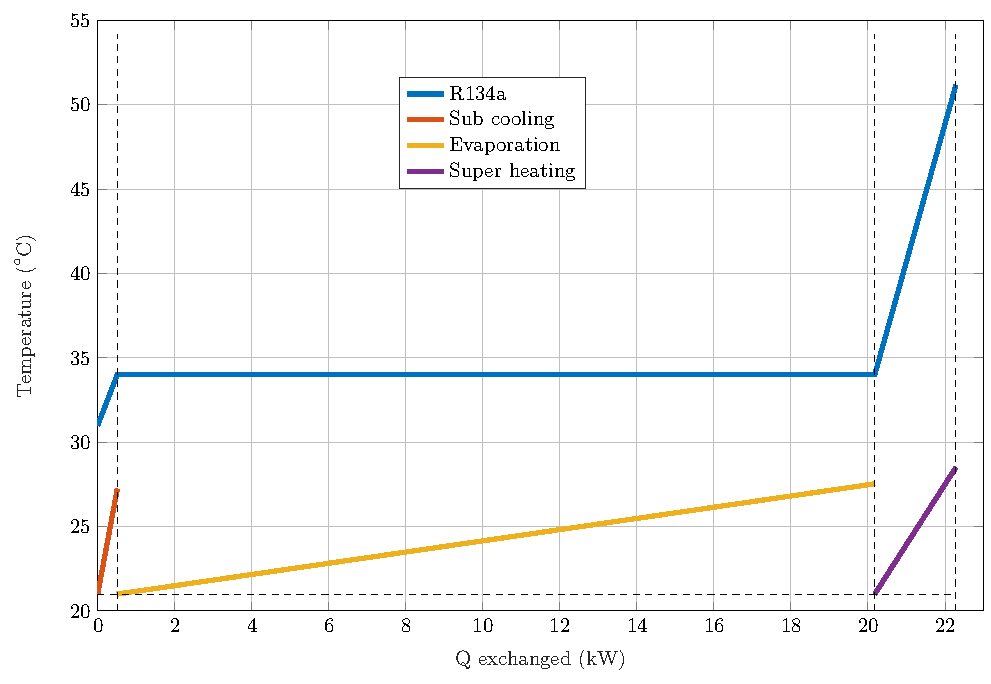
\includegraphics[width=0.8\textwidth]{plot_TQ_condenser}
\end{figure}

\section{Electrical power of the compressor and of the fan}
The electrical power of the compressor $\dot{W}_c$ is:
\begin{equation}
\Wdot{compressor} = \frac{\mdot{refrigerant} \cdot (\h{2} - \h{1})}{\eta_{m/e}} = \round{4.766862116669429e+03}\,W
\end{equation}
The fan power $\Wdot{fan}$ is:
\begin{equation}
\Wdot{fan} = \frac{\vdot{air} \cdot \Delta p}{\eta_{fan}} 
= \frac{\mdot{air} \cdot \Delta p}{\rho{air} \cdot \eta_{fan}} = \round{2.186714207745111e+02}\,W
\end{equation}
Where the pressure variation of the air side for each row is given by an experimental formula: $\Delta p_{\text{each row}} = 0.208 \cdot v_{air}^{1.87} = \round{1.622856357866490}\mmhoo$.
The total $\Delta p(Pa) = g \cdot \Delta p_{\text{each row}} \cdot \Nr = \round{47.760662612010812}\,Pa$

\section{Coefficient of performance (C.O.P.) of the cycle and of the overall plant}
The C.O.P. of the cycle is defined as the ratio between the \emph{useful refrigeration effect} and the \emph{compression power} (power transferred to the fluid by the compressor)
\begin{equation}
\cop{cycle} = \frac{\Qdot{u}}{\mdotdh{ref}{2}{1}} = \round{4.202804457126008}
\end{equation}
The overall (or total) C.O.P. of the refrigerator is defined as the ratio between the \emph{useful refrigeration effect} and the \emph{overall electrical consumption} of the refrigeration system (electrical power of the compressor and electrical power of the fan):
\begin{equation}
\cop{plant} = \frac{\Qdot{u}}{\mdotdh{ref}{2}{1}/\eta_{m/e} + \Wdot{fan}} = \round{3.539439107205700}
\end{equation}
Varying the condensation temperature $\Tcond$ we can plot the $\cop$ of the system, reported in figure \ref{fig:cop_tcond}.

\begin{figure}[H]
  \caption{$\cop$ function of the condensation temperature.}
  \label{fig:cop_tcond}
  \centering
    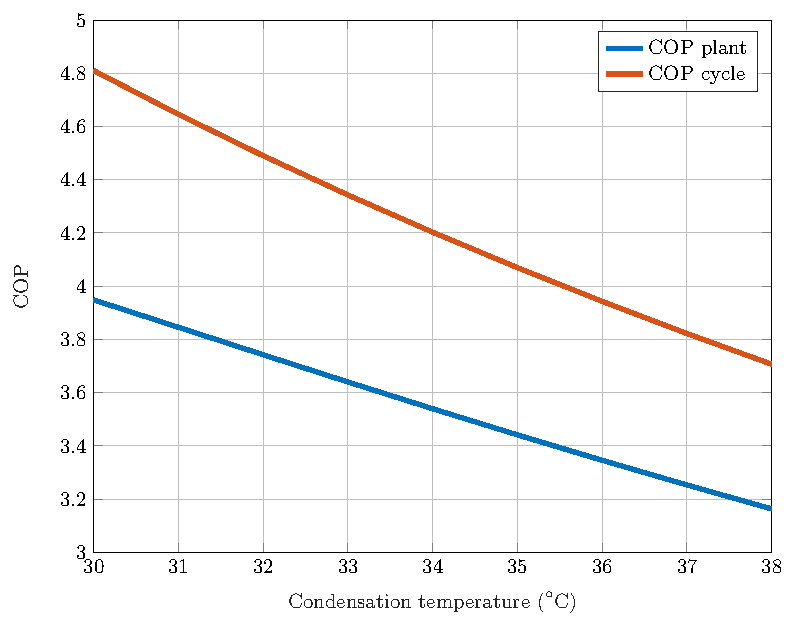
\includegraphics[width=0.8\textwidth]{plot_cop_tcond}
\end{figure}

\section{Double-throttling refrigeration cycle}
We make a change in the previous plant, in fact to improve the total word produced we make a double-throttling refrigeration cycle, that requires an additional valve, a separator of liquid and vapour and a two stage compressor. This is particularly feasible in case the system uses a multi-stage compressor instead of a volumetric one.
The new scheme is drawn in figure \ref{fig:plantB}
\begin{figure}[h]
  \caption{Double-throttling refrigeration Circuit Layout.}
  \label{fig:plantB}
  \centering
  \includegraphics[width=0.8\textwidth]{plant_double_fig}
\end{figure}

To evaluate the new $\cop$ is necessary to evaluate the thermodynamical conditions of the main point.
We must apply the same calculations for three different value of the separation pressure $\psep = 3\,bar,5\,bar,7\,bar$. Since the method is exactly the same we will explain it step by step just for  $\psep = 7\,bar$ and than show simply the results for the others.

\subsubsection*{Point 1)}
Point 1 is at \emph{compressor inlet}. We know its temperature $T_1=\Tevap + \Delta\T{SH}$ and its pressure exactly the evaporation pressure $p_1 = p{SAT}(\Tevap)$. With the two parameters of temperature and pressure we can evaluate with \md of R134a also entropy and enthalpy functions of temperature and pressure:
\[\begin{cases}{}
T_1 = \Tevap + \Delta\T{SH} = -4\celsius + 2\celsius = -2\celsius \\ 
p_1 = \p{SAT}(\Tevap) = \round{252675.641745724/100000}\,bar
\end{cases}\]
\pointdatatable{1}{271.15-273.15}{2.526756417457240}{398.0080526304495}{1.735915384972629}
%
%
%
\subsubsection*{Point 2)}
Point 2 is at \emph{high pressure compressor outlet}. We know its pressure $p_2=\psep$. We do not directly have the temperature $T_2$ but we can obtain it from the definition of efficiency of the compressor:
\begin{equation}
\label{eq:eta_highp_compressor_iso}
\eta_T^{isoentropic} = \frac{h_2^{IS}-h_1}{h_2-h_1} = 70\%
\end{equation}
We don't know $h_2^{IS}$ but we can compute it from point 1 to point $2^{IS}$ considering an \emph{isoentropic process}:
\[\begin{cases}{}
p_2^{IS} = p_2 = \round{7} \,bar \\ 
s_2^{IS} = s_1 = \round{1.735915384972629} \kjkgk
\end{cases}\]
Now we can obtain from \md $h_2^{IS} = h(p_2^{IS},\ s_2^{IS}) = \round{419341.755693655/1000} \kjkg$.
\\Reverting equation \ref{eq:eta_highp_compressor_iso} we can get $h_2$:
\begin{equation}
h_2=h_1- \frac{h_1 - h_2^{IS}}{\eta_T^{iso}} = \round{428484.771292172/1000} \kjkg
\end{equation}
With \md we finally evaluate $s_2 = s(p_2,\ h_2)$ and $T_2 = T(p_2,\ h_2)$ of point 2:
\pointdatatable{2}{314.913795703623-273.15}{7}{428484.771292172/1000}{1765.37699480870/1000}
%
%
%
\subsubsection*{Point 5)}
Point 5 is at \emph{condenser outlet}. We know its temperature $T_5=\Tcond - \Delta\T{SC}$ and its pressure exactly the condensation pressure $p_5 = \p{SAT}(\Tcond)$. With the two parameters of temperature and pressure we can evaluate with \md of R134a also entropy and enthalpy functions of temperature and pressure:
\pointdatatable{5}{304.15-273.15}{862625.775293017/100000}{243167.202571111/1000}{1148.00179566533/1000}
%
%
%
\subsubsection*{Point 6)}
Point 6 is at \emph{valve outlet}. We can model the valve as \emph{isoenthalpic} so we know enthalpy of point 6 as it is equal to point 5. Moreover we can consider that point 6 is also at separator inlet so it is at separation pressure $\psep$. With the two parameters of enthalpy and pressure we can evaluate with \md of R134a also entropy and temperature functions of enthalpy and pressure: 
\pointdatatablechi{6}{299.863248086079-273.15}{700000/100000}{243167.202571111/1000}{1148.59955084120/1000}{0.0350383107681397}
%
%
%
\subsubsection*{Point 7)}
Point 7 is at \emph{separator outlet} on the \emph{saturated liquid} side. The pressure is exactly separation pressure $\psep$. From these considerations we can easily get all the thermodynamical properties from the saturated liquid table of R134a.
\pointdatatable{7}{299.863248086079-273.15}{700000/100000}{236993.312583956/1000}{1128.01053225836/1000}
%
%
%
\subsubsection*{Point 8)}
Point 9 is at \emph{separation valve outlet}. We can model the valve as \emph{isoenthalpic} so we know enthalpy of point 9 as it is equal to point 8. Moreover we can consider that point 9 is also at evaporator inlet so it is at evaporation pressure $\pevap$. With the two parameters of enthalpy and pressure we can evaluate with \md of R134a also entropy and temperature functions of enthalpy and pressure: 
\pointdatatablechi{8}{269.15-273.15}{252675.641745724/100000}{236993.312583956/1000}{1137.70527718657/1000}{0.210043454039980}
%
%
%


\subsubsection*{Point 9)}
Point 9 is at \emph{separator outlet} on the \emph{saturated vapour} side. The pressure is exactly separation pressure $\psep$. From these considerations we can easily get all the thermodynamical properties from the saturated liquid table of R134a.
\pointdatatable{9}{299.863248086079-273.15}{700000/100000}{413197.297645036/1000}{1715.62500714225/1000}
%
%
%

\subsubsection*{Point 3)}
Point 3 is at \emph{low pressure turbine inlet}. Before entering into the turbine we have a mixing before flows 2 coming from the high pressure turbine and 9 that it is saturated vapour from the separator.
So we can set up energy and mass balance for the mixing:
\begin{numcases}{}
\mdoth{2} + \mdoth{9} = \mdoth{3}  \label{eq:mdoth3} \\ 
\mdot{2} + \mdot{9}  = \mdot{3}    \label{eq:mdot3}
\end{numcases}
We already know enthalpy of points 2 and 9, and we want to obtain $\h{3}$. 
From mass balance at the separator knowing the quality of point 6 $\chi_6$ we can get the relationship between the mass flow rates.
\begin{numcases}{}
\mdot{2} = \mdot{3} \cdot (1 - \chi_6) =  \round{ 0.112175245741141 * 1000}\E{-3} \kgs \label{eq:mdot2}\\
\mdot{9} = \mdot{3} \cdot \chi_6 = \round{0.004073147322459 * 1000}\E{-3} \kgs		   \label{eq:mdot9}
\end{numcases}
Replacing the value of mass flow rates $\mdot{2}$ and $\mdot{9}$ into equation \ref{eq:mdoth3} we can find $\h{3}$.
Since the mixing is considerable \emph{isobar} we know pressure of point 3 $\p{3}$ equal to separation pressure.
\[\begin{cases}{}
\p{3} = \psep = \round{7} \,bar \\ 
\h{3} = \round{4.279491240396638e+05/1000} \kjkg
\end{cases}\]
From enthalpy and pressure we can get all the thermodynamical properties from \md of R134a.
\pointdatatable{3}{314.377492868158-273.15}{700000/100000}{427949.124039664/1000}{1763.67461167085/1000}
%
%
%

We summarize all the thermodynamical conditions in the following table.
\subimport{tables/}{plantB}

\newpage
Now we can plot T-s and p-h diagrams.

\begin{figure}[H]
  \caption{T-s diagram.}
  \label{fig:ts_diagrammB}
  \centering
    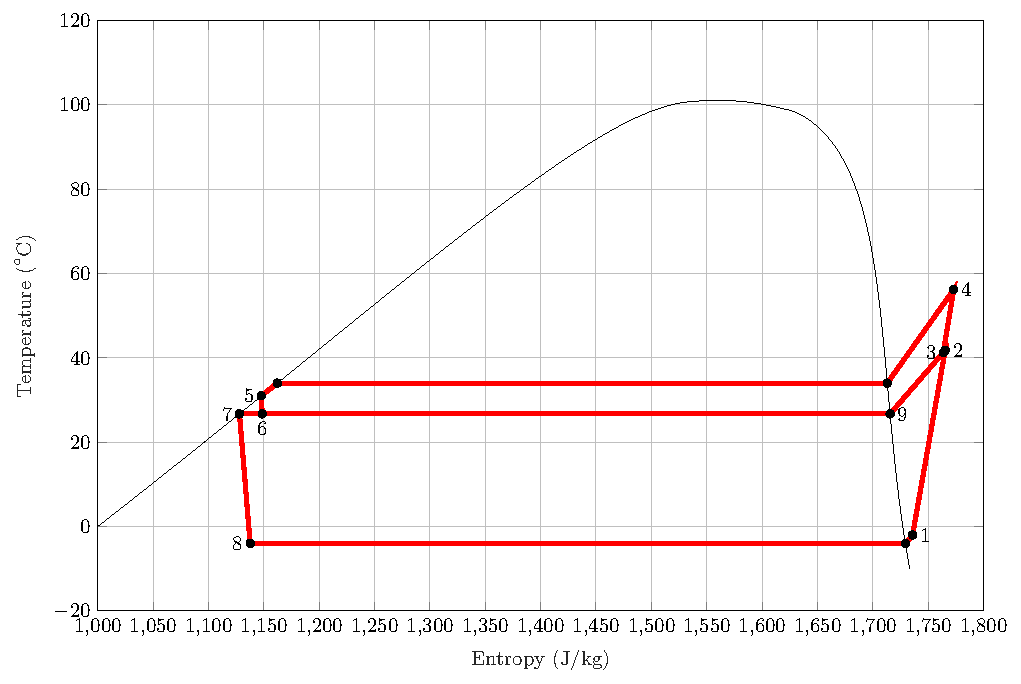
\includegraphics[width=0.8\textwidth]{plot_TS_caseB}
\end{figure}

\begin{figure}[H]
  \caption{p-h diagram.}
  \label{fig:ph_diagrammB}
  \centering
    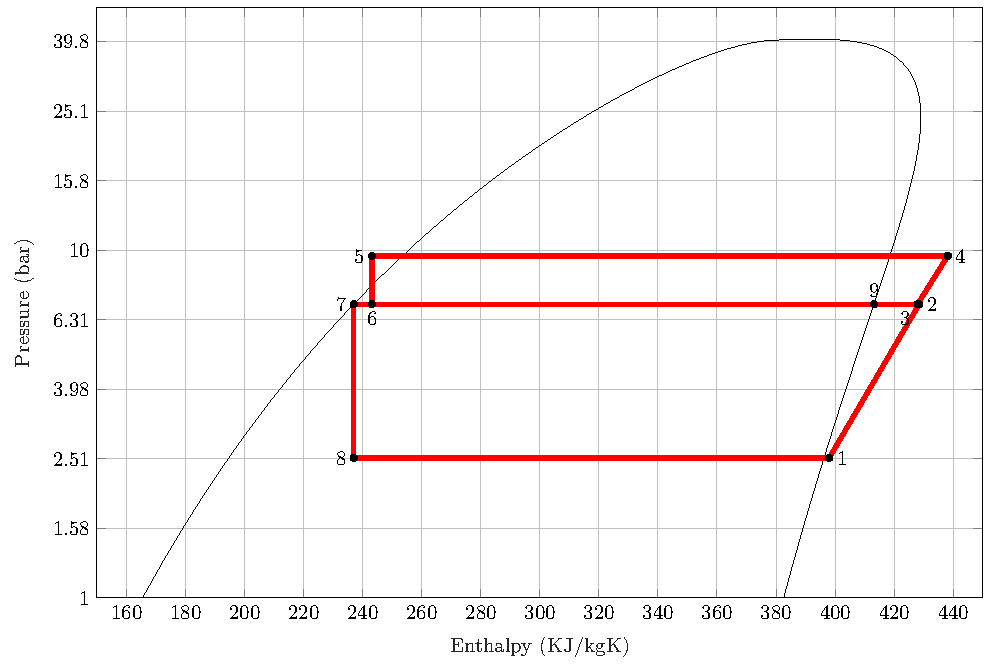
\includegraphics[width=0.8\textwidth]{plot_PH_caseB}
\end{figure}

\section{Coefficient of performance (C.O.P.) of the double-throttling cycle}
With the themodynamical conditions of each point of the plant we can evaluate the performance.
The C.O.P. of the cycle is defined as the ratio between the \emph{useful refrigeration effect} and the \emph{compression power} (power transferred to the fluid by the compressor)
\begin{equation}
\cop{cycle} = \frac{\Qdot{u}}{\mdotdh{ref}{2}{1}} = \round{4.290987436581633
}
\end{equation}
The overall (or total) C.O.P. of the refrigerator is defined as the ratio between the \emph{useful refrigeration effect} and the \emph{overall electrical consumption} of the refrigeration system (electrical power of the compressor and electrical power of the fan):
\begin{equation}
\cop{plant} = \frac{\Qdot{u}}{\mdotdh{ref}{2}{1}/\eta_{m/e} + \Wdot{fan}} = \round{3.610446076595549}
\end{equation}
Varying the separation pressure $\psep$ we can plot the $\cop$ of the system, reported in figure \ref{fig:cop_psep}.

\begin{figure}[H]
  \caption{$\cop$ function of the condensation temperature.}
  \label{fig:cop_psep}
  \centering
    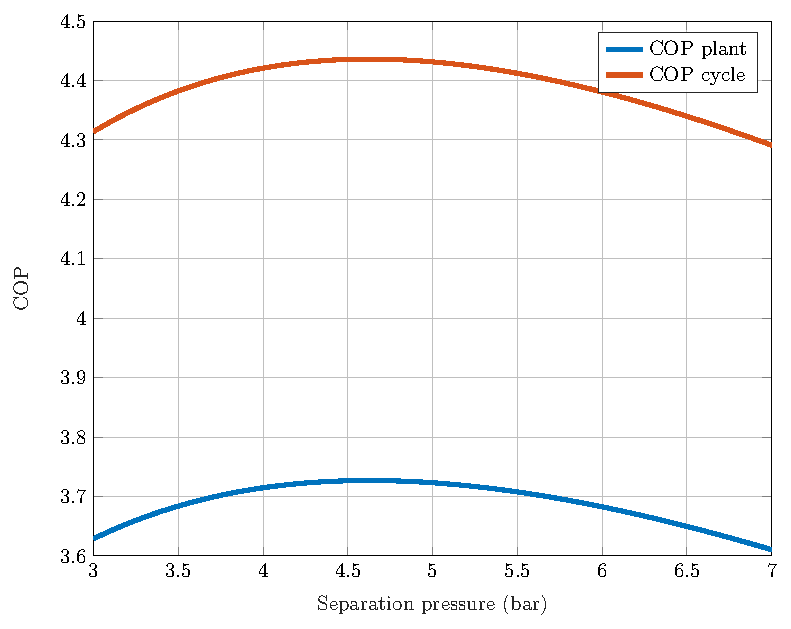
\includegraphics[width=0.8\textwidth]{plot_cop_psep}
\end{figure}

In figure \ref{fig:cop_psep} is interesting to notice that the $ \cop $ has a maximum value in correspondence of $\psep \approx 4.5\,bar$ for both the plant and the cycle. In case of design of the plant can be interesting to choose the right $\psep$ to maximize the performance of the cycle. 


\end{document}








